\documentclass[Analysis-3]{subfiles}

\begin{document}
\chapter*{Lecture 28} %Set chapter name
\addcontentsline{toc}{chapter}{Lecture 28} %Set chapter title
\setcounter{chapter}{28} %Set chapter counter
\setcounter{section}{0}
%The content
\section{Green's Theorem}
\begin{Thm}{$\R^2$ version of Green's Theorem}{}
    Let $\mathcal{R} \subseteq \R^2 $ be a simply connected domain with boundary curve $\mathcal{C}$ where parametrisation is taken in anti-clockwise direction. Let $\vec{F} = (P,Q)$ be a $\mathscr{C}^1$ vector field on $\mathcal{R}$, then 
\[
    \int_{\mathcal{C}} \vec{F} \cdot \dd r := \int_{\mathcal{C}} P \, \dd x + Q \, \dd y = \int_{\mathcal{R}} \left( \pdv{Q}{x} - \pdv{P}{y}\right) \dd A 
\]
\end{Thm}

\textit{Proof}.(for Simple region)

\begin{wrapfigure}{r}{0.50\textwidth}
    \centering
    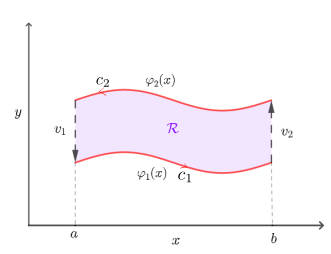
\includegraphics[width=.78\linewidth]{figures/lec-28.1.png}
    \caption{A simple region}
\end{wrapfigure}

\vspace{0.2cm}

 Let, $\mathcal{R} = \qty{(x,y) | a\le x\le b, \varphi_1(x) \le y \le \varphi_2(x)}$ be a simple region. Here $\mathcal{C} = c_1 \cup v_2 \cup c_2 \cup v_2$ is the curve bounding the region along anti-clockwise direction (as shown in the picture). 

 \begin{align*}
    -\int_{\mathcal{R}} \pdv{P}{y} \dd A &= -\int_{a}^{b} \int_{\varphi_1(x)}^{\varphi_2(x)} \pdv{P}{y} \dd y \dd x \\
    &= - \int_{a}^{b} (P(x,\varphi_2(x))-P(x,\varphi_1(x))) \dd x \\
 \end{align*}

 Now, $c_1,c_2,v_1,v_2$ can be explicitly written as, 
 \begin{align*}
    v_1 &= \qty{(a,t) | \varphi_1(a) \le t \le \varphi_2(a)} \\
    c_1 &= \qty{(x,\varphi_1(x)) | a \le x \le b} \\
    v_2 &= \qty{(a,t) | \varphi_1(b) \le t \le \varphi_2(b)} \\
    c_2 &= \qty{(x,\varphi_2(x)) | a \le x \le b}
 \end{align*}

 Now,

 \begin{align*}
    \int_{v_1} P \dd x &= \int_{v_1} P(x(t),y(t)) \dv{x(t)}{t} \dd t = 0 \\
    \int_{c_1} P \dd x &= \int_{a}^{b} P(t,\varphi_1(t)) \dd t \\
    \int_{c_2} P \dd x &= \int_{a}^{b} P(t,\varphi_2(t)) \dd t \\
    \implies \int_{\mathcal{C}} P\dd x &= -\int_{\mathcal{R}} \pdv{P}{y} \dd A
 \end{align*}

 
 By similar mechanism we can show $\int_{\mathcal{C}} Q \dd y = \int_{\mathcal{R}} \pdv{Q}{y} \dd A$. The resst follows from here. $\hfill \blacksquare$


 \end{document}